\documentclass[12pt, a4paper]{article}
\usepackage[utf8]{inputenc}
\usepackage[czech]{babel}
\usepackage[T1]{fontenc}
\usepackage{graphicx}
\usepackage{amsmath, amssymb, amsthm}
\usepackage[margin=2.5cm]{geometry}
\usepackage{url}
\usepackage{tabularx}
\usepackage{float}

\begin{document}

\begin{titlepage}
    \begin{center}
        {\large {Přírodovědecká fakulta}} \\
        \vspace{3mm}
        {\large Univerzita Karlova}
        
        \vspace{15mm}
        
\includegraphics[width=0.5\linewidth]{img/PrFUK_strom_digital_cerna.png} 
        \vfill{}
        
        {\huge\bfseries Výpočet souřadnic bodů v rovině Křovákova zobrazení} \\
        \vspace{5mm}
        {\large {Matematická kartografie}} \\
        \vfill
        
        \begin{center}
            \large Teodor Sorokáč \\
        \end{center}
        \vfill{}

        \begin{center}
            \ 2. N-GKDPZ \\
            \ Praha 2026
        \end{center}
        
    \end{center}
\end{titlepage}

\newpage
\section{Zadání}

\vspace{5mm}
\subsection*{\textbf{Úloha č. 1: Výpočet souřadnic bodů v rovině Křovákova zobrazení}}

\vspace{3mm}
GPS aparaturou změřte zeměpisné souřadnice bodů $P_{1}$ a $P_{2}$ vztažené k elipsoidu WGS-84 a vypočtěte jejich obraz v rovině Křovákova zobrazení. Měření proveďte na bodech o známých souřadnicích (trigonometrický bod), a to opakovaně. 
\vspace{3mm}

\noindent Pro transformaci mezi elipsoidy použijte sedmiprvkovou Helmertovu prostorovou podobnostní transformaci danou vztahem:
\vspace{3mm}

\[
\begin{pmatrix}
X \\
Y \\
Z
\end{pmatrix} 
= m 
\begin{pmatrix}
1 & \omega_{z} & -\omega_{y} \\
-\omega_{z} & 1 & \omega_{x} \\
\omega_{y} & -\omega_{x} & 1
\end{pmatrix}
\begin{pmatrix}
X^{\prime} \\
Y^{\prime} \\
Z^{\prime}
\end{pmatrix}
+ 
\begin{pmatrix}
\Delta X \\
\Delta Y \\
\Delta Z
\end{pmatrix}.
\]

\vspace{3mm}
\noindent Parametry prostorové transformace jsou definovány následovně:
\begin{itemize}
    \item $\omega_{x} = 4.9984^{\prime\prime}$
    \item $\omega_{y} = 1.5867^{\prime\prime}$
    \item $\omega_{z} = 5.2611^{\prime\prime}$
    \item $m - 1 = -3.5623 \cdot 10^{-6}$
    \item $\Delta X = -570.8285 \text{ m}$
    \item $\Delta Y = -85.6769 \text{ m}$
    \item $\Delta Z = -462.8420 \text{ m}$
\end{itemize}
\vspace{3mm}

\noindent Určení zeměpisné šířky obrazu bodu $P$ na Besselově elipsoidu proveďte s~přesností $0.001^{\prime\prime}$. Souřadnice obrazu bodu $P$ v~rovině Křovákova zobrazení určete s~přesností na cm. V~bodech $P_{1}$ a $P_{2}$ dále vypočtěte:
\begin{itemize}
    \item hodnoty délkového zkreslení $m-1$,
    \item hodnoty meridiánové konvergence $c$.
\end{itemize}
\vspace{3mm}

\noindent Volitelně porovnejte účinek zanedbání změny/vlivu elipsoidu na souřadnice bodů $P_{1}$, $P_{2}$ a na vzdálenosti $\lVert P_{1}-P_{2} \rVert$. Jak se budou lišit takto určené souřadnice a vzdálenosti od hodnot vztažených k~elipsoidu WGS-84?
\vspace{3mm}

\noindent Obrazy bodů $P_{1}$, $P_{2}$ a jejich blízkého okolí vizualizujte s~použitím vhodných podkladových geografických dat (např. WMS). Výpočty realizujte v~SW Matlab.

\vspace{10mm}
\subsection*{\textbf{Hodnocení:}}

\begin{center}
\resizebox{\textwidth}{!}{
\begin{tabular}{|l|c|}
\hline
\textbf{Krok}                                                                         & \textbf{Hodnocení} \\ [0.5ex]  \hline\hline
\rule{0pt}{3ex} Výpočet souřadnic bodu v rovině Křovákova zobrazení + zkreslení.                 &  20b                \\ \hline
\rule{0pt}{3ex}\textit{Výpočet meridiánové konvergence.}                                        &  \textit{+5b}      \\ \hline
\rule{0pt}{3ex}\textit{Zanedbání změny elipsoidu: souřadnice měřeny na Besselově elipsoidu.}    &  \textit{+5b}      \\ \hline
\rule{0pt}{3ex}\textit{Zanedbání vlivu elipsoidu: souřadnice měřeny na Gaussově kouli.}         &  \textit{+5b}      \\ \hline
\rule{0pt}{3ex}\textit{Transformace $(\varphi,\lambda,H)\rightarrow(Y,X,Z)$.}                          &  \textit{+10b}     \\ \hline
\rule{0pt}{3ex}\textit{Použití dotransformace (přesnost 2cm).}                                  &  \textit{+15b}     \\ \hline
\rule{0pt}{3ex}\textbf{Max celkem:}                                                             & \textbf{60b}       \\ \hline
\end{tabular}
}
\end{center}
\vspace{15mm}

\subsection*{Řešené bonusové úlohy}
V rámci úlohy byly vypracované následující bonusové úlohy: \textit{Výpočet meridiánové konvergence (+5b), Zanedbání změny elipsoidu: souřadnice měřeny na Besselově elipsoidu (+5b), Zanedbání vlivu elipsoidu: souřadnice měřeny na Gaussově kouli (+5b), Transformace $(\varphi,\lambda,H)\rightarrow(Y,X,Z)$ (+10b).}

\newpage
\section{Úvod do problematiky úlohy}
Převod bodu ze systému zeměpisných souřadnic vztažených k výchozímu referenčnímu elipsoidu (WGS-84) do systému pravoúhlých souřadnic Křovákova zobrazení (S-JTSK) lze rozdělit do několika fází:
\subsection*{Zeměpisné a geocentrické souřadnice}
Prostorové geocentrické souřadnice $(X, Y, Z)$ bodu na referenčním elipsoidu o souřadnicích $(\varphi, \lambda)$ se určí pomocí příčného poloměru křivosti $N$:

\[ X = N \cos \varphi \cos \lambda \]

\[ Y = N \cos \varphi \sin \lambda \]

\[ Z = N (1 - e^2) \sin \varphi \]
\vspace{3mm}

\noindent Zpětný převod pro zeměpisnou délku $\lambda$ vychází přímo z podílu os $Y$ a $X$:
\vspace{3mm}

\[ \tan \lambda = \frac{Y}{X} \]
\vspace{3mm}

\noindent Zeměpisná šířka $\varphi$ se odvodí ze součtu čtverců prvních dvou rovnic ($X^2 + Y^2 = N^2 \cos^2 \varphi$) a následného podílu se souřadnicí $Z$:
\vspace{3mm}

\[ \sqrt{X^2 + Y^2} = N \cos \varphi \]
\vspace{3mm}

\[ \frac{Z}{\sqrt{X^2 + Y^2}} = \frac{N (1 - e^2) \sin \varphi}{N \cos \varphi} = (1 - e^2) \tan \varphi \]
\vspace{3mm}

\[ \tan \varphi = \frac{Z}{(1 - e^2)\sqrt{X^2 + Y^2}} \]


\newpage
\section*{Helmertova prostorová transformace}
\vspace{5mm}
Pro převod souřadnic mezi geocentrickými systémy (např. z WGS-84 na Besselův elipsoid) se využívá sedmiprvková Helmertova transformace. Transformace je definována jakožto posun ($\Delta X, \Delta Y, \Delta Z$), rotace ($\omega_x, \omega_y, \omega_z$) a měřítkovým koeficientem ($m$):

\[ P = m R P' + \Delta \]
\vspace{3mm}

\noindent Celková matice rotace $R$ vznikne součinem rotačních matic každé osy ($R = R_x \cdot R_y \cdot R_z$):

\[ R_x = \begin{pmatrix} 1 & 0 & 0 \\ 0 & \cos \omega_x & \sin \omega_x \\ 0 & -\sin \omega_x & \cos \omega_x \end{pmatrix} \]
\vspace{3mm}

\[ R_y = \begin{pmatrix} \cos \omega_y & 0 & -\sin \omega_y \\ 0 & 1 & 0 \\ \sin \omega_y & 0 & \cos \omega_y \end{pmatrix} \]
\vspace{3mm}

\[ R_z = \begin{pmatrix} \cos \omega_z & \sin \omega_z & 0 \\ -\sin \omega_z & \cos \omega_z & 0 \\ 0 & 0 & 1 \end{pmatrix} \]
\vspace{3mm}

\noindent Výsledná transformační rovnice má pak tento tvar:

\[ \begin{pmatrix} X \\ Y \\ Z \end{pmatrix} = m \begin{pmatrix} 1 & \omega_z & -\omega_y \\ -\omega_z & 1 & \omega_x \\ \omega_y & -\omega_x & 1 \end{pmatrix} \begin{pmatrix} X' \\ Y' \\ Z' \end{pmatrix} + \begin{pmatrix} \Delta X \\ \Delta Y \\ \Delta Z \end{pmatrix} \]

\newpage
\section*{Křovákovo zobrazení}
\vspace{5mm}
Křovákovo zobrazení je kombinací dvou zobrazení. Z Elipsoidu na kouli pomocí Gaussova konformního zobrazení a poté pomocí Lambertova konformního kuželového zobrazení do roviny. Elipsoid, který využívá je Besselův elipsoid ($a = 6377397.155$ m, $b = 6356078.9633$ m) a pomocnou referenční plochou je Gaussova koule ($R = 6380703.6105$ m).

\vspace{3mm}
\noindent Nejprve se zeměpisné souřadnice Besselova elipsoidu $(\varphi, \lambda)$ zobrazí na Gaussovu kouli $(u, v)$ pomocí konstant zobrazení ($\alpha, k$):

\[ \tan\left(\frac{u}{2} + 45^\circ\right) = \frac{1}{k} \left( \tan\left(\frac{\varphi}{2} + 45^\circ\right) \left( \frac{1 - e \sin \varphi}{1 + e \sin \varphi} \right)^{\frac{e}{2}} \right)^\alpha \]
\vspace{3mm}

\[ v = \alpha \cdot (\lambda + 17^\circ 40') \]
\vspace{3mm}

\noindent Pomocí sférické trigonometrie se tyto souřadnice přepočítají na kartografické souřadnice $(s, d)$ k definovanému pólu $(u_k, v_k)$, a zobrazení se tak převede do obecné polohy:

\[ \sin s = \sin u \sin u_k + \cos u \cos u_k \cos(v_k - v) \]
\vspace{3mm}

\[ \sin d = \frac{\cos u}{\cos s} \sin(v_k - v) \]
\vspace{3mm}

\noindent Pomocí Lambertova kuželového konformního zobrazení, kterým se Gaussova koule promítne do roviny, se získají polární souřadnice $(\rho, \epsilon)$ s využitím konstanty kužele $c$ a poloměru základní rovnoběžky $\rho_0$:

\[ \rho = \rho_0 \left( \frac{\tan(\frac{s_0}{2} + 45^\circ)}{\tan(\frac{s}{2} + 45^\circ)} \right)^c \]
\vspace{3mm}

\[ \epsilon = c \cdot d \]
\vspace{3mm}

\noindent Výsledné polární souřadnice se nakonec převedou na pravoúhlé souřadnice $x$ a $y$ pomocí následujícího vztahu:

\[ x = \rho \cos \epsilon \]
\vspace{3mm}

\[ y = \rho \sin \epsilon \]

\section*{Délkové zkreslení a meridiánová konvergence}
\vspace{5mm}
Měřítko délek $m$ lze vypočítat pomocí vztahu:

\[ m = \frac{c\rho}{R \cos s} \]
\vspace{3mm}

\noindent Meridiánová konvergence $c$ (úhel mezi obrazem místního a základního poledníku) se určí z rozdílu úhlů:

\[ c = \epsilon - \xi \]

\newpage
\section*{Výsledky}
\vspace{5mm}
Vstupní data pro výpočet tvořily zeměpisné souřadnice dvou bodů ($P_1, P_2$) zaměřené v systému WGS-84. Výpočty jednotlivých kroků, byly provedeny v programu python. Souřadnice bodů ($P_1, P_2$) byly nejprve pomocí Helmertovy transformace převedeny na Besselův elipsoid a následně Křovákovým zobrazením transformovány do rovinných souřadnic S-JTSK.
\vspace{5mm}

\noindent Pro posouzení vlivu referenčního tělesa byly vytvořeny tři skripty: převod z WGS-84 (\textit{WGSToJTSK.py}), výpočet se zanedbáním změny elipsoidu (\textit{bessToJTSK.py}) a zjednodušený výpočet na Gaussově kouli v rámci zanedbání vlivu elipsoidu (\textit{sphereToJTSK.py}). Déle bylo spočítáno v obou bodech ($P_1, P_2$) délkové zkreslení $m$ a meridiánová konvergence $c$. 

\vspace{3mm}
\noindent V následujících tabulkách jsou prezentovány výsledky transformací a výpočtů. \textit{Tabulka 1} shrnuje vypočtené souřadnice bodů v rovině Křovákova zobrazení v porovnání s daty ČÚZK. \textit{Tabulka 2} uvádí hodnoty délkového zkreslení a meridiánové konvergence. \textit{Tabulka 3} zobrazuje rozdíly souřadnic a vzdáleností zjednodušených metod.
\vspace{10mm}

\begin{table}[htpb]
\centering
\footnotesize
\setlength{\tabcolsep}{4pt}
\begin{tabular}{|c|c|c|c|c|c|c|c|c|}
  \hline
  & \multicolumn{2}{c|}{\textbf{WGS-84}} & \multicolumn{2}{c|}{\textbf{Bessel}} & \multicolumn{2}{c|}{\textbf{Sféra}} & \multicolumn{2}{c|}{\textbf{ČÚZK}} \\ \hline
  \textbf{Bod} & $X \ [m]$ & $Y \ [m]$ & $X \ [m]$ & $Y \ [m]$ & $X \ [m]$ & $Y \ [m]$ & $X \ [m]$ & $Y \ [m]$ \\ \hline
  \textbf{P1} & 1074826.06 & 717457.40 & 1074896.80 & 717548.77 & 1070242.43 & 718341.02 & 1074826.11 & 717457.41 \\ \hline
  \textbf{P2} & 1071417.87 & 712249.19 & 1071488.82 & 712341.34 & 1066829.45 & 713138.69 & 1071417.85 & 712249.00 \\ \hline
\end{tabular}
\caption{Vypočtené souřadnice bodů P1 a P2}
\end{table}

\vspace{3mm}

\begin{table}[htpb]
\centering
\footnotesize
\setlength{\tabcolsep}{6pt}
\begin{tabular}{|c|c|c|c|c|c|c|}
  \hline
   & \multicolumn{2}{c|}{\textbf{WGS-84 $\rightarrow$ JTSK}} & \multicolumn{2}{c|}{\textbf{Bessel $\rightarrow$ JTSK}} & \multicolumn{2}{c|}{\textbf{Sféra $\rightarrow$ JTSK}} \\ \hline
   \textbf{Bod} & $m \ [-]$ & $c \ [rad]$ & $m \ [-]$ & $c \ [rad]$ & $m \ [-]$ & $c \ [rad]$ \\ \hline
   \textbf{P1} & 0.999900 & -0.1312 & 0.999900 & -0.1313 & 0.999901 & -0.1315 \\ \hline
   \textbf{P2} & 0.999902 & -0.1304 & 0.999902 & -0.1304 & 0.999903 & -0.1306 \\ \hline
\end{tabular}
\caption{Délkové zkreslení a meridiánová konvergence bodů}
\end{table}
\vspace{3mm}

\begin{table}[htpb]
\centering
\footnotesize
\setlength{\tabcolsep}{5pt}
\begin{tabular}{|c|c|c|c|c|c|c|} \hline
      & \multicolumn{2}{c|}{\textbf{P1}} & \multicolumn{2}{c|}{\textbf{P2}} & \multicolumn{2}{c|}{}\\ \hline
      \textbf{Metoda} & $\Delta X \ [m]$ & $\Delta Y \ [m]$ & $\Delta X \ [m]$ & $\Delta Y \ [m]$ & $d \ [m]$ & $\Delta d \ [m]$ \\ \hline
     \textbf{WGS-84 $\rightarrow$ JTSK} & - & - & - & - & 6224.24 & - \\ \hline
     \textbf{Bessel $\rightarrow$ JTSK} & 70.74 & 91.37 & 70.95 & 92.15 & 6223.48 & -0.76 \\ \hline
     \textbf{Sféra $\rightarrow$ JTSK} & -4583.63 & 883.62 & -4588.42 & 889.50 & 6221.95 & -2.29 \\ \hline
     \textbf{ČÚZK} & 0.05 & 0.01 & -0.02 & -0.19 & 6224.22 & -0.02 \\ \hline
\end{tabular}
\caption{Rozdíly souřadnic a vzdáleností bodů vzhledem k plné transformaci z WGS-84}
\end{table}

\section{Zhodnocení výsledků a závěr}
\vspace{5mm}
Z dosažených výsledků (viz \textit{Tabulka 3}) je patrný zásadní vliv volby referenčního tělesa na určení konečných souřadnic. Plná transformace z WGS-84 dosahuje nejvyšší přesnosti. Zatímco zanedbání změny elipsoidu patrně ovlivňuje polohovou přesnost na úrovni desítek metrů. Zanedbáním vlivu elipsoidu dochází k nejhorším výsledkům a to až do řádu kilometrů. Oproti tomu hodnoty délkového zkreslení a meridiánové konvergence zůstávají napříč všemi metodami téměř bezezměny. 

\begin{figure}[htpb]
    \centering
    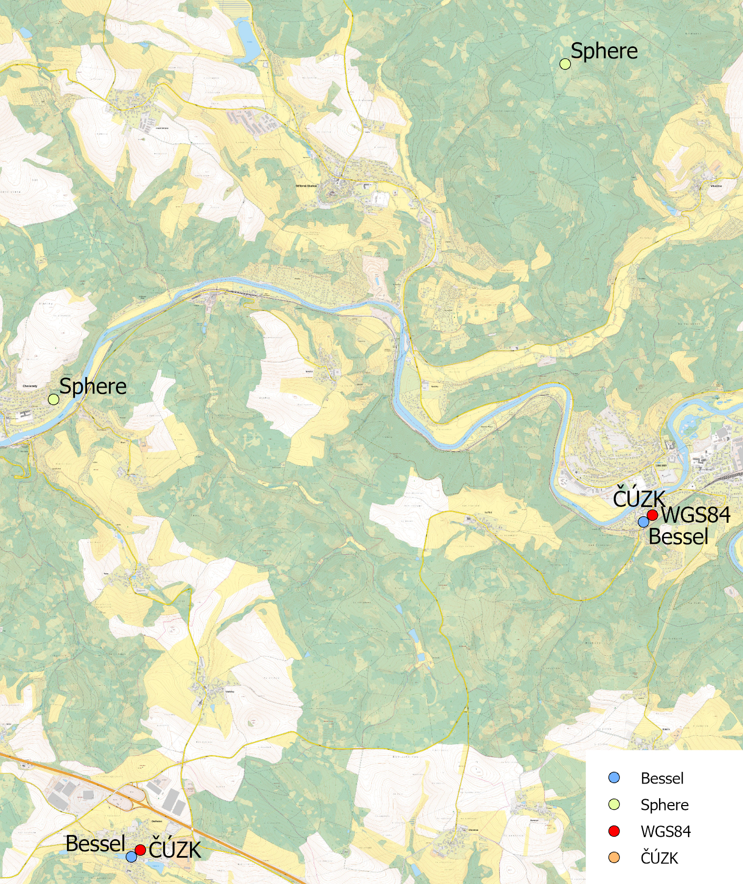
\includegraphics[width=0.5\textwidth]{img/mapa_u1.png} 
    \caption{Vizualizace transformovaných bodů a referenčních dat ČÚZK}
    \label{fig:mapa_arcgis}
\end{figure}

\vspace{3mm}
\noindent Cílem úlohy byla transformace souřadnic dvou bodů z referenčního systému WGS-84 do roviny Křovákova zobrazení (S-JTSK). K provedení výpočtů byl využit skriptovací jazyk Python. Součástí řešení bylo také určení délkového zkreslení a meridiánové konvergence pro oba body. Z porovnání výsledků vyplývá, že zanedbání transformace mezi referenčními elipsoidy (WGS-84 a Besselovým) způsobuje polohovou chybu v řádu desítek metrů. Úplné zanedbání zploštění Země a náhrada elipsoidu referenční koulí pak vede k odchylkám až v řádu kilometrů. Oproti tomu hodnoty meridiánové konvergence a délkového zkreslení se při použití těchto zjednodušených metod mění jen minimálně a vliv volby referenčního tělesa je na ně prakticky zanedbatelný.

\newpage
\section*{Seznam literatury}
\vspace{5mm}

\noindent Český úřad zeměměřický a katastrální (ČÚZK). (2026): \textit{Geoportál ČÚZK} [online]. Praha. Dostupné z: \texttt{https://geoportal.cuzk.cz/} [cit. 30. 5. 2026].
\vspace{3mm}

\noindent ESRI. (2026): \textit{ArcGIS Pro Documentation} [online]. Redlands, CA: Environmental Systems Research Institute. Dostupné z: \texttt{https://pro.arcgis.com/} [cit. 30. 5. 2026].
\vspace{3mm}

\noindent BAYER, T. (2025): \textit{Transformace zeměpisných souřadnic mezi elipsoidy (stručný návod k úloze 1)}. Výukový materiál pro předmět Matematická kartografie, Katedra aplikované geoinformatiky a kartografie, Přírodovědecká fakulta UK [cit. 30. 5. 2025].
\vspace{3mm}

\end{document}